\documentclass[11pt]{article}
\usepackage[margin=0.75in]{geometry}
\usepackage{graphicx}
\usepackage{booktabs}
\usepackage{hyperref}
\title{Source-reconciled phase accounting for four genus-2 follow-ups}
\author{aburan28/crypto research packet}
\date{25 October 2026}
\begin{document}
\maketitle

This is a derived view of the frozen public known-answer cohort. It does not
execute a collector or change a measured cost. The native Rust normalizer
reads the source JSONL records and the review packet's standardized targets.
Every available candidate and rho phase sum is checked against its recorded
representative cold total. All 6,120 priced aggregate method cells are also
checked against the standardized 36-cell grid. The 12,850 standardized target
rows produce 23,176 reconciled candidate/rho method rows; 1,264 rows carry
explicit null candidate costs (1,260 coordinate-only Kummer gates and four
pencil cap outcomes).

\begin{figure}[h]
\centering
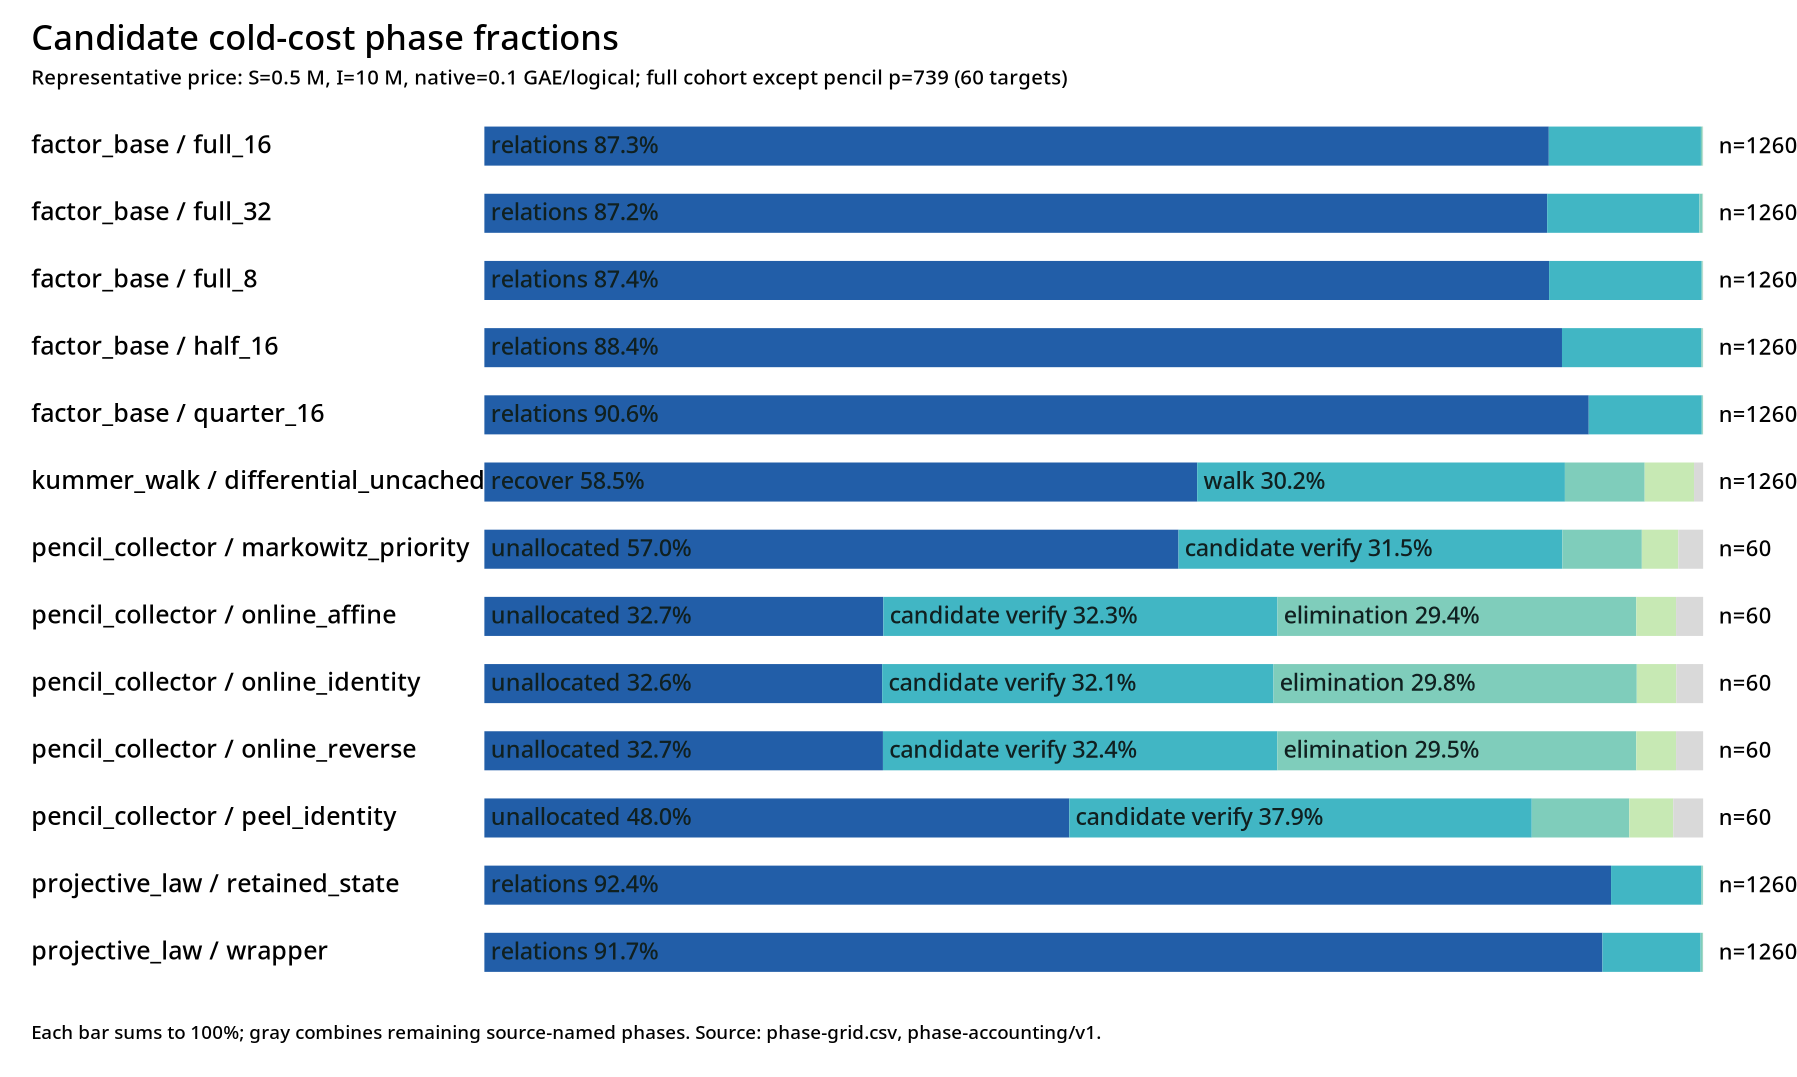
\includegraphics[width=\textwidth]{phase-fractions.png}
\caption{Recorded candidate cold-cost fractions at $S/M=0.5$, $I/M=10$,
native $=0.1$ GAE per logical operation. All factor-base, projective-law, and
Kummer arms cover 1,260 targets. Pencil bars show their observed $p=739$
subcohort of 60 verified targets per arm. Source phase names are retained.
Gray combines the phases outside each bar's four largest.}
\end{figure}

\section*{Accounting boundary}
The denominator is the matched source addition in each study. The candidate
and rho costs include the cold setup and source verification charged by the
source validators. Where a source supplied counters but no phase assignment,
the corresponding bar is labeled \texttt{unallocated}; no step is inferred.
The pencil rho phase array omits source verification, which is retained as a
checked residual. Kummer rho supplies one unphased total. The original
point-driven pencil cohort remains incomplete: 543 distinct targets have a
verified candidate solve, one has cap-only records, and 716 have no candidate
record. No 1,260-target pencil cost ratio is inferred here.

\section*{Review files}
\begin{itemize}
\item \texttt{phase-targets.csv}: target-level candidate and rho phase rows at
the representative price, with source paths and explicit nulls;
\item \texttt{phase-grid.csv}: per-arm, slice, method and phase rows for all
36 price cells, with sums, target counts and cold-cost fractions;
\item \texttt{summary.json}: schema, reconciliation counts and price cell;
\item \texttt{render.py}, \texttt{phase-fractions.svg}: editable graph source.
\end{itemize}
Rebuild with \texttt{cargo run --release --locked --offline --bin normalize\_phases}
from the review crate, then run \texttt{python3 phase-accounting/render.py}.
The normalizer source is in the review crate's \texttt{src/bin} directory.
\end{document}
